\chapter{EM-CCD camera calibration}
\section{Andor Basic code listing for automatic image acquisition}
\label{sec:basic-acquisition}
\definecolor{light-gray}{gray}{0.95}

\lstdefinestyle{myframe}{
  basicstyle=\LSTfont,
  % basicstyle=\footnotesize\ttfamily,
  rulesepcolor=\color{gray} ,
  rulecolor = \color{black},
  frame = single,
  % framerule = 0pt,
  backgroundcolor =\color{light-gray}, 
  fontadjust=true,
  breaklines = true,
  showstringspaces=false,
}
\lstdefinestyle{mybasic}{
  language=[Visual]Basic,
  commentstyle=\itshape,
  style=myframe
}
\lstdefinestyle{mypython}{
  language=Python,
  showstringspaces=false,
  tabsize=4,
  commentstyle=\itshape,
  basicstyle=\ttfamily,
  morekeywords={models, lambda, forms},
  frame = single,
  breaklines = true,
  style=myframe
}


\begin{lstlisting}[style=mybasic]
' This is code for the Basic interpreter in Andor Solis
function ~GetSaturatingExposure()
        SetKineticNumber(1)
        exp=.01
        SetExposureTime(exp)
        run()
        m=maximum(#0,1,512)
        GetSaturatingExposure=exp*10000/(m-100)
        CloseWindow(#0)
return
name$ = "C:\Users\work\Desktop\martin\20111111\scan-em3\ixon_"
print("start")

SetOutputAmp(1)
print("conv_start")
exp= ~GetSaturatingExposure()
print(exp)
SetExposureTime(exp)
SetKineticNumber(20)
SetShutter(0,1)
run()
save(#0,name$ + "conv1_dark.sif")
ExportTiff(#0, name$ + "conv1_dark.tif", 1, 1, 0, 0)
CloseWindow(#0)
CloseWindow(#1)
        
SetShutter(1,1)
run()
save(#0,name$ + "conv1_bright.sif")
ExportTiff(#0, name$ + "conv1 _bright.tif", 1, 1, 0, 0)
CloseWindow(#0)
CloseWindow(#1)

SetOutputAmp(0)
SetShutter(1,1)
for i = 40 to 300 step 10
        SetGain(i)
        exp=~GetSaturatingExposure()
        print(exp)
        SetExposureTime(exp)
        SetKineticNumber(20)
        SetShutter(0,1)
        run()
        save(#0,name$ + str$(i) + "_dark.sif")
        ExportTiff(#0, name$ + str$(i) + "_dark.tif", 1, 1, 0, 0)
        CloseWindow(#0)
        CloseWindow(#1)
        SetShutter(1,1)
        run()
        save(#0,name$ + str$(i) + "_bright.sif")
        ExportTiff(#0, name$ + str$(i) + "_bright.tif", 1, 1, 0, 0)
        CloseWindow(#0)
        CloseWindow(#1)
next

SetOutputAmp(1)
print("conv_end")
exp= ~GetSaturatingExposure()
print(exp)
SetExposureTime(exp)
SetKineticNumber(20)
SetShutter(0,1)
run()
save(#0,name$ + "conv2_dark.sif")
ExportTiff(#0, name$ + "conv2_dark.tif", 1, 1, 0, 0)
CloseWindow(#0)
CloseWindow(#1)
        
SetShutter(1,1)
run()
save(#0,name$ + "conv2_bright.sif")
ExportTiff(#0, name$ + "conv2 _bright.tif", 1, 1, 0, 0)
CloseWindow(#0)
CloseWindow(#1)
\end{lstlisting}

\begin{table}[!htbp]
  \centering
%  \begin{tabular}{|l|l|l|l|l|l|l|l|}
  \begin{tabular}{r l l r  l r l}
\hline
$\textsf{gain}_\textrm{software}$ & $1/(M\cdot M_\textrm{pre})$ & $N_r$ & $N_{(M)}/(W\times H)$ &  \textsf{exposure} & $N_{(M)}'/(W\times H)$ & $1/F_n$ \\
 & [e/ADU] & [e/px] & [e/px] & [ADU] & [s] & [e/(px s)]  \\
\hline
conv1 & 1.3165 & 7.189 & 3008.66      & 0.2016 & 14923 & 0.981 \\
50 & 0.1160 & 0.486 & 260.05 & 0.0289 & 8995 & 0.591 \\
60 & 0.0984 & 0.406 & 225.46 & 0.0249 & 9054 & 0.595 \\
70 & 0.0841 & 0.349 & 190.52 & 0.0212 & 8983 & 0.591 \\
80 & 0.0729 & 0.305 & 165.24 & 0.0186 & 8907 & 0.586 \\
90 & 0.0680 & 0.288 & 150.54 & 0.0161 & 9368 & 0.616 \\
100 & 0.0611 & 0.262 & 128.47 & 0.0136 & 9427 & 0.620 \\
110 & 0.0550 & 0.241 & 121.11 & 0.0129 & 9409 & 0.619 \\
120 & 0.0510 & 0.228 & 113.71 & 0.0120 & 9498 & 0.624 \\
130 & 0.0465 & 0.211 & 106.66 & 0.0112 & 9541 & 0.627 \\
140 & 0.0433 & 0.201 & 96.95 & 0.0101 & 9564 & 0.629 \\
150 & 0.0405 & 0.192 & 89.68 & 0.0093 & 9671 & 0.636 \\
160 & 0.0380 & 0.183 & 87.24 & 0.0090 & 9656 & 0.635 \\
170 & 0.0359 & 0.175 & 81.56 & 0.0084 & 9739 & 0.640 \\
180 & 0.0339 & 0.169 & 79.80 & 0.0081 & 9863 & 0.648 \\
190 & 0.0321 & 0.163 & 74.00 & 0.0075 & 9806 & 0.645 \\
200 & 0.0305 & 0.158 & 72.57 & 0.0073 & 9878 & 0.649 \\
210 & 0.0292 & 0.155 & 69.44 & 0.0070 & 9944 & 0.654 \\
220 & 0.0280 & 0.150 & 67.69 & 0.0068 & 9971 & 0.656 \\
230 & 0.0268 & 0.147 & 65.63 & 0.0065 & 10057 & 0.661 \\
240 & 0.0257 & 0.188 & 63.90 & 0.0063 & 10131 & 0.666 \\
250 & 0.0244 & 0.140 & 62.52 & 0.0062 & 10026 & 0.659 \\
260 & 0.0237 & 0.137 & 62.86 & 0.0062 & 10078 & 0.663 \\
270 & 0.0229 & 0.135 & 63.17 & 0.0062 & 10130 & 0.666 \\
280 & 0.0221 & 0.133 & 63.64 & 0.0062 & 10204 & 0.671 \\
290 & 0.0214 & 0.130 & 63.38 & 0.0062 & 10162 & 0.668 \\
300 & 0.0205 & 0.128 & 63.20 & 0.0062 & 10133 & 0.666 \\
conv2 & 1.5953 & 8.768 & 8198.86 & 0.5291 & 15496 & 1.019 \\
\hline
\end{tabular}
%  \includegraphics[width=12cm]{../app_cam/ixon3}
\caption{Comparison of read noise for different EM-gain settings
  (first column) of the Andor IXon3. $W$ and $H$ are the size of the sensor (in pixels). The value $N_{(M)}'$
  estimates the number of photoelectrons the detector would have
  seen with \unit[1]{s} integration time and is used to calculate
  the excess noise factor in the last column. In EM-mode the fastest
  readout speed was used \unit[10]{MHz} with vertical shift speed of
  \unit[1.7]{$\mu$s}.}
  \label{tab:ixon-table}
\end{table}

\newpage

\section{Python code listing for the read noise evaluation}
\label{sec:python-readnoise-eval}

\begin{figure}
  \centering
  \pdfinput{17cm}{ixon_conv1}
  \pdfinput{17cm}{ixon_300}
  \caption{Readnoise evaluation using the Python code in section
    \ref{sec:python-readnoise-eval}{\bf top:} Conventional readout of
    an Andor IXon3 camera. {\bf bottom:} readout with an EM-gain
    setting of 300 on the same camera with identical sample. {\bf
      left:} 2D histogram of per pixel variances against binned
    intensities. {\bf middle:} variance of 20 dark images. {\bf
      right:} mean of 20 dark images.}
  \label{fig:ixon}
\end{figure}
  


\begin{lstlisting}[style=mypython]
#!/usr/bin/env python
# ./ti.py /media/backup/andor-ultra-ixon/martin/20111111/scan-em3/ ultra 2700
import sys
import os

import matplotlib
matplotlib.use('Agg')

from pylab import *
from libtiff import TIFFfile, TIFFimage
from scipy import stats

seterr(divide='ignore')

folder = sys.argv[1]
cam = sys.argv[2]
gain = sys.argv[3]

def readpics(gain,cam='ixon_',isdark=False):
    print 'loading ', os.path.join(folder,cam) + '_' + gain + '_bright.tif'
    fg=TIFFfile(os.path.join(folder,cam) + '_' + gain + '_bright.tif')
    bright,bright_names=fg.get_samples()
    bg=TIFFfile(os.path.join(folder,cam) + '_' + gain + '_dark.tif')    
    dark,dark_names=bg.get_samples()
    return (bright[0],dark[0])

(f,b) = readpics(gain=gain,cam=cam)

bg=mean(b,axis=0)
v=var(f,axis=0)
i=mean(f,axis=0)

ny,nx=64,128
H,y,x=histogram2d(v.flatten(),i.flatten(),bins=[ny,nx],
                  range=[[0,v.max()],[0,i.max()]])
extent = [x[0], x[-1], y[0], y[-1]] 
acc=zeros(x.shape,dtype=float64)
accn=zeros(x.shape,dtype=int64)
s=nx/i.max()
for ii,vv in nditer([i,v]):
    p=round(ii*s)
    acc[p]+=vv
    accn[p]+=1   

fig=figure(figsize=(24, 8),dpi=300)
hold(False)
title('bal')
subplot(1,3,1)
imshow(log(H), extent=extent,
           aspect='auto', interpolation='none',origin='lower')
hold(True)
ax=x[nonzero(accn)]
ay=acc/accn
ay=ay[nonzero(accn)]
l=round(.6*len(ax))
bx=ax[0:l]
by=ay[0:l]
plot(ax,ay,'r+')
slope,intercept,rval,pval,stderr=stats.linregress(bx,by)
plot(ax,polyval([slope,intercept],ax))
xlabel('intensity/ADU')
ylabel(r'variance/ADU$^2$')
real_gain=1/slope # unit electrons/ADU
read_noise=sqrt(var(b))*real_gain # electrons RMS per pixel
mean_elecs=(mean(f)-mean(b))*real_gain # photoelectrons electrons per pixel
print gain,cam,real_gain,read_noise,mean_elecs,mean(b),rval,pval,stderr
tit='EM-gain: %s, cam: %s, real gain: %.2f e/ADU\n
read noise: %.2f e RMS/pixel, mean: %.2f e/pixel, offset: %.2f'
% (gain,cam,real_gain,read_noise,mean_elecs,mean(b))
title(tit)
subplot(1,3,2)
imshow(var(b,axis=0))
title('variance of darkimages')
colorbar()
subplot(1,3,3)
imshow(mean(b,axis=0))
title('mean of darkimages')
colorbar()
show()
fig.savefig(cam+'_'+gain+'.png')
\end{lstlisting}


\chapter{Optical sectioning by structured illumination}
\comment{
\jpginput{}{m_phase}{}
}


\begin{figure}[H]
  \centering
  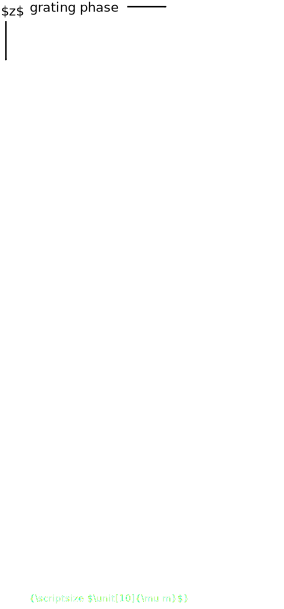
\includegraphics[height=.9\textheight]{m_phase}
  \caption{Structured illumination images of the same of the beads
    from \figref{fig:m_wf}. Of each $z-$slice (rows) four exposures
    with different grating phase (columns) were captured.}
  \label{fig:m_phase}
\end{figure}
